\subsubsection{\theoryC{Axion-like particles at the HL-LHC and the HE-LHC}}
\contributors{M.~Low, A.~Mariotti, D.~Redigolo, F.~Sala, K.~Tobioka}\rt{There are comments to address.}
%\textbf{Matthew Low$^a$, Alberto Mariotti$^b$, Diego Redigolo$^c$, Filippo Sala$^d$, Kohsaku Tobioka$^e$}~\\ ~\\
%\textit{\small $^a$ School of Natural Sciences, Institute for Advanced Study, Einstein Drive, Princeton, NJ 08540, USA,\\
%$^b$Theoretische Natuurkunde and IIHE/ELEM, Vrije Universiteit Brussel, and International,\\
%Solvay Institutes, Pleinlaan 2, B-1050 Brussels, Belgium\\
%$^c$School of Natural Sciences, Institute for Advanced Study, Einstein Drive, Princeton, NJ 08540, USA,\\
%Raymond and Beverly Sackler School of Physics and Astronomy, Tel-Aviv University, Tel-Aviv 69978, Israel,\\
%Department of Particle Physics and Astrophysics, Weizmann Institute of Science, Rehovot 7610001,Israel\\
%$^d$ DESY, Notkestra{\ss}e 85, D-22607 Hamburg, Germany\\
%$^e$C.N. Yang Institute for Theoretical Physics, Stony Brook University, Stony Brook, NY 11794-3800\\}

%\subsubsection{Setup and Motivation}
%\paragraph*{Setup and Motivation}

The main focus of this contribution is future search strategies for axion-like particles (ALPs) in the mass range between 1 and 90 GeV.  For simplicity we consider an ALP, $a$, that couples only to gauge bosons, including a non-zero coupling to gluons.
We call this type of ALP a ``KSVZ-ALP'' because it is inspired by the simplest QCD axion model~\cite{Peccei:1977hh,Kim:1979if,Shifman:1979if}.
Such an ALP is perhaps the most theoretically compelling case and also the natural target for hadron colliders, such as the HL- and HE-LHC.  The effective Lagrangian for the KSVZ-ALP, below the $Z$ mass, is
%
\begin{align}
\mathcal{L}_{\text{int}}&= \frac{a}{4\pi f_a}\left[ \alpha_s c_3 G^a\tilde{G}^a+ \alpha_2 c_2 W^i\tilde{W}^i+ \alpha_1 c_1 B\tilde{B}\right],
\label{eq:LaFFdual}\\
&= \frac{a}{4\pi f_a}\left[ \alpha_s c_3 G^a\tilde{G}^a\!+ \alpha_{\text{em}} c_{\gamma} F\tilde{F}\!+\!2\alpha_2 c_W W^{-}\tilde{W}^{+}\!+\!\frac{2\alpha_{\text{em}}}{t_w} c_{Z\gamma} Z\tilde{F}\!+\alpha_2 c_w^2 c_{Z} Z\tilde{Z}\right]\,,\label{eq:La123}
\end{align}
%
where $\tilde{F}^{\mu\nu}=(1/2)\,\epsilon^{\mu\nu\rho\sigma}F_{\rho\sigma}$ for any field strength, $\alpha_1=(5/3)\, \alpha'$ is the GUT-normalized $U(1)_Y$ coupling constant, and $t_w=s_w/c_w$ where $c_w^2=1-s_w^2=m_W^2/m_Z^2$.  The coefficients $c_i$ encode the Adler-Bell-Jackiw (ABJ) anomalies of the global $U(1)$ symmetry (of which the ALP is the pseudo-Goldstone boson) with $SU(3)$ and $SU(2)\times U(1)_Y$.
After EWSB, one can write
%
\begin{equation}
c_{\gamma}=c_2+\frac{5}{3}c_1,\quad c_W=c_2, \quad c_Z=c_2+t_w^4\frac{5}{3} c_1, \quad c_{Z\gamma}=c_2-t_w^2\frac{5}{3} c_1  .
\end{equation}
%
For $m_a \lesssim m_Z$, the relevant two-body decays of $a$ are to two photons and to two jets, with widths
%
\begin{equation} \label{eq:widths}
\Gamma_{gg}=\frac{K_g\alpha_s^2c_3^2}{8 \pi^3}  \frac{m_a^3}{f_a^2},
\qquad \Gamma_{\gamma\gamma}=\frac{\alpha_{\text{em}}^2c_\gamma^2}{64 \pi^3}  \frac{m_a^3}{f_a^2},
\end{equation}
%
where
$K_g=2.1$ includes higher-order QCD corrections~\cite{Djouadi:2005gj}.
The couplings in \eq{eq:LaFFdual} can be generated by heavy vector-like fermions with a mass at $g_* f_a$, where $g_*$ can be as large as $4\pi$.
Explicit realisations include: i) KSVZ ``heavy axion'' models where the axion potential is UV-dominated, the axion mass is heavier than expected from QCD contributions alone, and the decay constant, $f_a$, can be as low as a TeV (see e.g. \citerefs{Berezhiani:2000gh,Hook:2014cda,Fukuda:2015ana,Dimopoulos:2016lvn,Agrawal:2017ksf});
ii) ALPs arising in standard paradigms addressing the EW hierarchy problem, such as SUSY, where spontaneous SUSY-breaking below \Mpl predicts, on general grounds, the existence of an $R$-axion~\cite{Nelson:1993nf,Bellazzini:2017neg}.

%\subsubsection{Present bounds}
%\paragraph*{Present bounds}
\begin{figure*}[t]
\centering
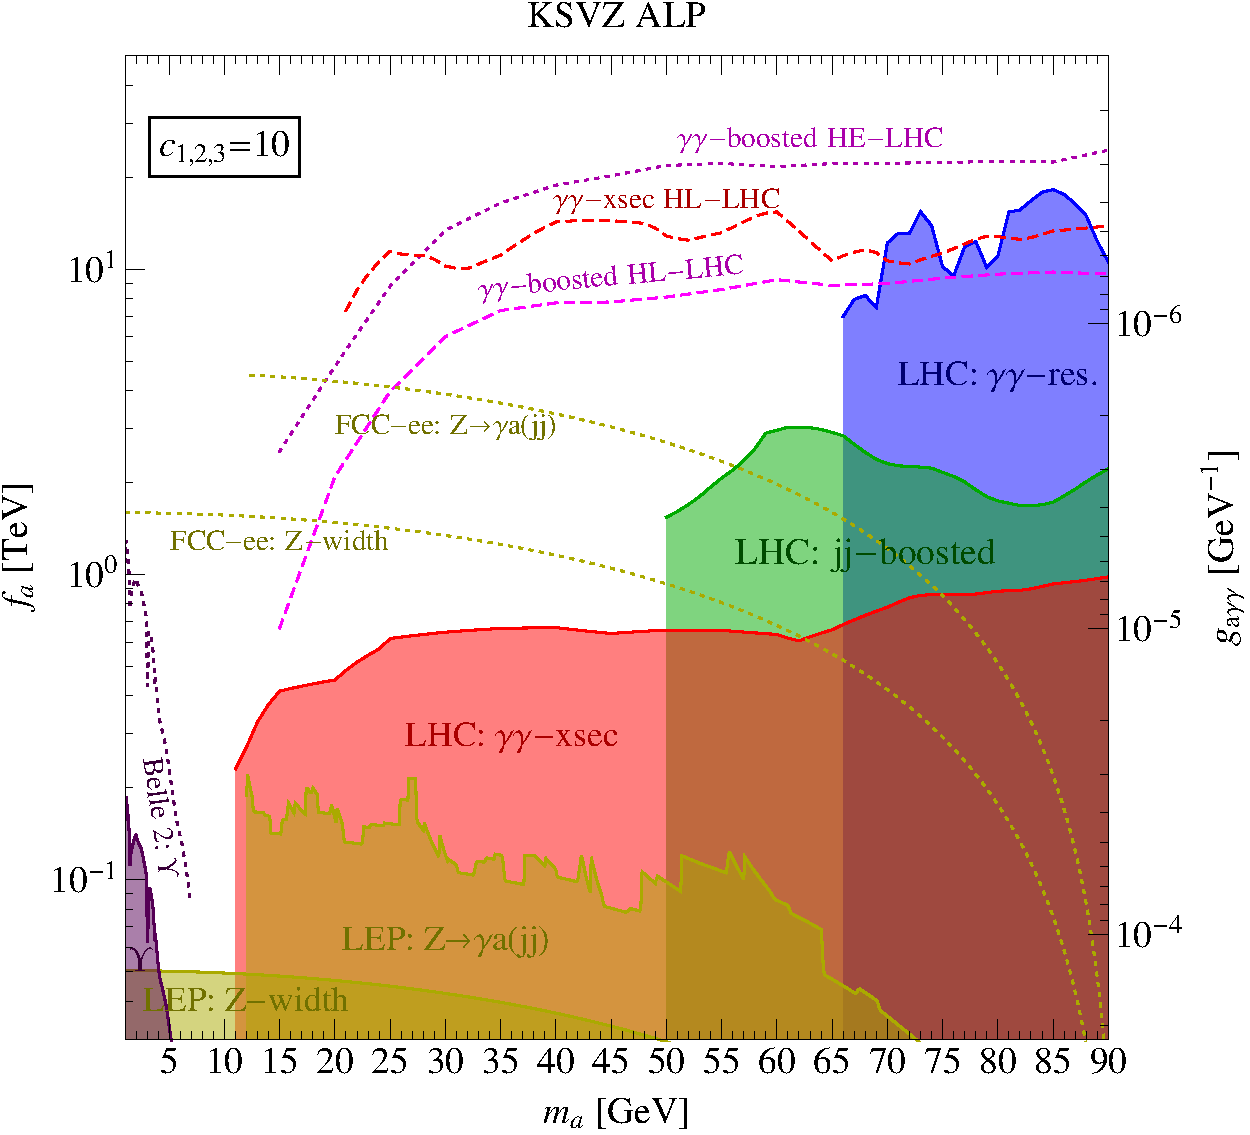
\includegraphics[scale=0.5]{\main/section7OtherSignatures/img/status.pdf}
\caption{
Status of the current best experimental constraints on the KSVZ-ALP with ABJ anomalies $c_{1,2,3}=10$. We include: Babar bound on $\Upsilon\to \gamma a(jj)$~\cite{Lees:2011wb} (purple) and its rescaling at Belle II~\cite{Riccardo:772} (purple dotted);  LEP searches of $Z\to \gamma a(jj)$~\cite{Adriani:1992zm} and constraints from the $Z$-width~\cite{Patrignani:2016xqp} (yellow) along with both of their rescalings at FCC-ee~\cite{Koratzinos:2015ywz} (yellow dotted); constraints from inclusive cross section measurements at the Tevatron~\cite{Aaltonen:2012jd} and the LHC~\cite{Aad:2012tba,Chatrchyan:2014fsa,Aaboud:2017vol} derived in \citeref{Mariotti:2017vtv} (red), and the rescaled sensitivities of the 8 TeV cross section measurement in \citeref{Aaboud:2017vol} at the HL-LHC (dashed red); LHC bounds on boosted dijet resonances~\cite{Sirunyan:2017nvi} reinterpreted for an ALP in \citeref{Mariotti:2017vtv} (green); LHC searches for diphoton resonances~\cite{Aad:2014ioa,CMS:2015ocq,CMS:2017yta} (blue); sensitivity of the boosted diphoton resonance search based on the monojet trigger at the HL-LHC with 3 ab$^{-1}$ and the HE-LHC with 12 ab$^{-1}$ (dashed/dotted magenta). In the right $y$-axis the scale is $ g_{a\gamma\gamma}\equiv(\alpha_{\text{em}}c_\gamma)/(\pi f_a c_3)$ to make contact with the QCD axion notation.}
\label{fig:status}
\end{figure*}

Barring a huge hierarchy among the anomaly coefficients, $c_{1,2} \gtrsim 10^2 c_3$, the width into gluons dominates over the one into photons, $\Gamma_{\gamma}/\Gamma_{gg}=\alpha_{\text{em}}^2/(8K_g\alpha_3^2) \sim 10^{-4}$.
ALPs that couple to gluons decay promptly in any kinematical configuration and mass range of interest for the LHC.
When accounting for the gluon coupling, searches based on rare decays of SM particles (Higgs, $Z$, $\Upsilon$, and $B$-mesons) into ALPs have a weaker bound on $f_a$ because the dominant branching ratio of the ALP is now into hadronic final states,
while the searches look for final states with muons or photons.
%%%
The only two relevant decay processes for our parameter space are $Z\to\gamma a$ and $\Upsilon_X\to \gamma a$, and the corresponding decay widths are given by
%
\begin{align}
&\Gamma(Z\to\gamma a)= \frac{\alpha_{\text{em}}^2c_{Z\gamma}^2}{96\pi^2t_w^2}\frac{m_Z^3}{f_a^2}\left(1-\frac{m_a^2}{m_Z^2}\right)^3 \ , \label{eq:Z}\\
&\Gamma(\Upsilon_X\to \gamma a)= \frac{\alpha_{\text{em}}c_{\gamma\gamma}^2}{2\pi}\left(\frac{m_{\Upsilon_X}}{4\pi f_a}\right)^2\left(1-\frac{m_a^2}{m_{\Upsilon_X}^2}\right)^3\Gamma(\Upsilon_X\to ll)\ ,\label{eq:upsilon}
\end{align}
%
where $\Gamma(\Upsilon_X\to ll)=\Gamma_{\Upsilon_X}\cdot \text{BR} (\Upsilon_X\to ll)$, $\text{BR} (\Upsilon_{2S,3S}\to ll)\simeq3.84\,,4.36\%$ and $\Gamma_{\Upsilon_{2S,3S}}\simeq20,32\text{ keV}$.
These constraints, together with those from the LHC, are shown in \fig{fig:status}.


The bound arising from the $Z$ decay in \eq{eq:Z} is based on the LEP search in \citeref{Adriani:1992zm} which has sensitivity down to 12 GeV.  In this range, this search is more powerful than the inclusive bound from the total $Z$-width~\cite{Patrignani:2016xqp}.  The bound coming from the $\Upsilon$ decay in \eq{eq:upsilon}, is based on BABAR data~\cite{Lees:2011wb} corresponding to $1.21\cdot 10^8$ $\Upsilon_{3S}$ and $0.98\cdot 10^8$  $\Upsilon_{2S}$.
``Standard'' inclusive diphoton resonance searches at the LHC do not probe masses below 65 GeV~\cite{Aad:2014ioa,CMS:2015ocq,CMS:2017yta}.

A first example of what can be done to improve the low mass reach is the CMS search for a dijet resonance recoiling against a hard jet~\cite{Sirunyan:2017nvi}, that we rescale here for an ALP produced in gluon fusion (see \citeref{Mariotti:2017vtv} for more details). As we see in \fig{fig:status}, this probes ALPs down to 50 GeV.
A second example is the bound from inclusive cross section measurements, derived in \citeref{Mariotti:2017vtv}, that reaches masses of 10~GeV.
References \cite{Aaltonen:2012jd,Aad:2012tba,Aaboud:2017vol,Chatrchyan:2014fsa} provide tables of the measured differential diphoton cross section per invariant mass bin, $\text{d}\sigma_{\gamma\gamma}/\text{d} m_{\gamma\gamma}$, with the relative statistical ($\Delta_{\rm stat}$) and systematical ($\Delta_{\rm sys}$) uncertainties.
%
A conservative bound was derived in \citeref{Mariotti:2017vtv} assuming zero knowledge of the background and requiring
\begin{equation}
\sigma^{\text{th}}_{\gamma\gamma}(m_a)<\left[m_{\gamma\gamma}^{\rm Bin}\cdot \frac{\text{d}\sigma_{\gamma\gamma}}{\text{d} m_{\gamma\gamma}}\cdot(1+ 2\Delta_{\rm tot})\right] \cdot \frac{1}{\epsilon_S (m_a)}.
\label{eq:sensitivity}
\end{equation}
where $\Delta_{\text{tot}}=\sqrt{\Delta_{\rm stat}^2+\Delta_{\rm sys}^2}$.
The signal efficiency $\epsilon_S (m_a)$ (see~\citeref{Mariotti:2017vtv} for its computation) does not go to zero below  $p_{T_{\gamma_1}}^{\text{min}}+p_{T_{\gamma_2}}^{\text{min}}$  because the ALP can still pass the cuts recoiling against unvetoed jet activity in the diphoton cross section measurements.
A lower limit on the invariant mass that can be measured, and thus on the testable $m_a$, is set~by
\begin{equation}
m_{\gamma\gamma}> \Delta R_{\gamma\gamma}^{\text{iso}}\sqrt{p_{T_{\gamma_1}}^{\text{min}}p_{T_{\gamma_2}}^{\text{min}}}\,,
\end{equation}
where $p_{T_{\gamma_{1,2}}}^{\text{min}}$ are the minimal cuts on the photon transverse momenta,
and $\Delta R_{\gamma\gamma}^{\text{iso}}=0.4$ is the standard isolation requirement between the photons.

%\subsubsection{Prospects for the HL-LHC and the HE-LHC}
%\paragraph*{Prospects for the HL-LHC and the HE-LHC}

We now discuss new LHC search strategies
for the HL-LHC and the HE-LHC to improve the coverage in the $f_a$-$m_a$ plane of KSVZ-like ALPs.
%
The reaches of future experiments are summarized as dashed lines in \fig{fig:status},
where we also display, for comparison, the Belle II and FCC-ee projections.\footnote{The Belle II and FCC-ee lines are obtained by rescaling of the present bounds from Babar and LEP with the future luminosities of these experiments: $2.8\cdot 10^{11}$ $\Upsilon_{2S}$s and $1.5\cdot 10^{11}$  $\Upsilon_{3S}$s for Belle II and $10^{12}$ $Z$s for FCC-ee.}

We show the reach of the HL-LHC from
inclusive cross section measurements
with the strategy outlined above,
assuming the same diphoton trigger as in the 8 TeV run. Our signal cross section includes matching up to 2 jets and a K-factor accounting for NLO corrections computed with ggHiggs v3.5~\cite{Ball:2013bra,Bonvini:2014jma,Bonvini:2016frm,Ahmed:2016otz} which includes full NNLO and approximate $\text{N}^3\text{LO}$ corrections plus threshold resummation at $\text{N}^3\text{LL}'$. The error on the sensitivity is assumed to be dominated by the error on the measurements.
In other words, we assume the MC uncertainties will be reduced below $\Delta_{\rm tot}$ (note that, at the present moment, MC uncertainties on the low-mass bins are at the level of 40\% using \sherpa~\cite{Aaboud:2017vol, Gleisberg:2008ta,Catani:2018krb}).
An unexplored direction in diphoton resonance searches is to reduce the photon isolation requirements and pass the trigger making the resonance recoiling against a hard jet.  In \fig{fig:status} we show the sensitivity at the HL-LHC and the HE-LHC of a search based on this idea.
The signal events are required to pass the existing monojet trigger (the leading jet with $p_{T_{j_1}}>500\text{ GeV}$ and $|\eta_{j_1}|<2.5$). As a consequence the two photons produced from the boosted ALP are collimated: $\Delta R_{\gamma\gamma}\simeq 2 m_a /p_{T_{j_1}} \lesssim 0.2\left(m_a/{\rm 50~GeV}\right)$ where $p_{T_{\gamma}}\sim p_{T_{j_1}}/2$. To improve $S/\sqrt{B}$ we then require $p_{T_{\gamma_{1,2}}}>120\text{ GeV}$ and $\Delta R_{\gamma\gamma}<0.8$ and bin the events in invariant mass bins with a constant width of 10 GeV. Since two photons fall into one isolation cone, $\Delta R_{\gamma\gamma}^{\text{iso}}=0.4$, standard photon isolation vetoes the ALP signal. In order to access lower invariant masses, we modify the standard isolation requirement by simply subtracting the hardest photon ($\gamma_1$) in the isolation cone of every test photon,  ($\gamma_{\rm test}\neq \gamma_1$). We require\footnote{$E_{T}^{\rm iso}$ is usually calculated using calorimeter cells, while here we also include information of charged tracks. Objects with $E_{T_i}<0.5$~GeV are not included in the sum~\cite{deFavereau:2013fsa}.}
\begin{equation}
%E_{T}^{\rm modiso}\equiv 
E_{T}^{\rm iso}-E_{T_{\gamma_1}}<{\rm 10~GeV}
\quad {\rm  where}\quad
E_{T}^{\rm iso}\equiv \sum_{i\neq \gamma_{\rm test}}^{\Delta R_{i,\gamma_{\rm test}}<0.4} E_{T_i} \ . \label{eq:newiso}
\end{equation}
%
To validate our analysis we first checked that the standard isolation with $E_{T}^{\rm iso}<$10~GeV in \delphes\, can reproduce the photon fake rate from multijets and the real photon acceptance from the SM Higgs decay, given by \citeref{ATL-PHYS-PUB-2016-026}. We find that the isolation in \eq{eq:newiso} gives a similar fake rate and real photon acceptance to the standard ones, while the photons from boosted ALP decays now pass the isolation. The modified isolation requirement allows us to go down to two-photon angular separation of $\Delta R\sim0.1$.\footnote{As minimal angular resolution we take for reference the square towers in the Layer 2 region of ATLAS ECAL~\cite{Aaboud:2016yuq}.} Below this value the two photon showers will start to overlap and the photon identification will have to be modified~\cite{Ellis:2012sd,Ellis:2012zp}.

To estimate the sensitivities in \fig{fig:status} we simulated the SM background from $2\gamma+n j$, matched for $n=1,2$, and from $j\gamma+j$ with a jet faking a photon both at 14 and 27 TeV. We expect the background from  $jj+j$ with two jets faking two photons to be subdominant.

%\subsubsection{Conclusions}
%\paragraph*{Conclusions}
In conclusion, we showed how the sensitivity to KSVZ ALPs can be greatly improved at the HL-LHC and the HE-LHC. Both experiments have a sensitivity that exceeds the one of FCC-ee. The type of searches discussed here will probe the parameter space of ``heavy axion'' models solving the strong CP-problem of the SM and probe SUSY scales, $g_{\ast} f_a$, as high as 100 TeV \emph{independently} of any particular assumption on the structure of the SUSY spectrum.

Our results have a broader application than the ones discussed here.  For example, they can still be the strongest probe in ALP scenarios where the ALP also couples to fermions and the SM Higgs, such as in composite Higgs models~\cite{Ferretti:2013kya,Cacciapaglia:2017iws} where the couplings to photons and gluons are, in fact, generated by top loops. Last but not least, the invariant mass sensitivity can likely be further extended to lower masses by studying to what extent the two collimated photons themselves can trip the monophoton trigger~\cite{toappear}, or developing techniques to perform bump hunts with L1 triggers~\cite{Collaboration:2283192}.






